\documentclass[tikz, border=2pt]{standalone}
\usepackage{amsmath}

\begin{document}
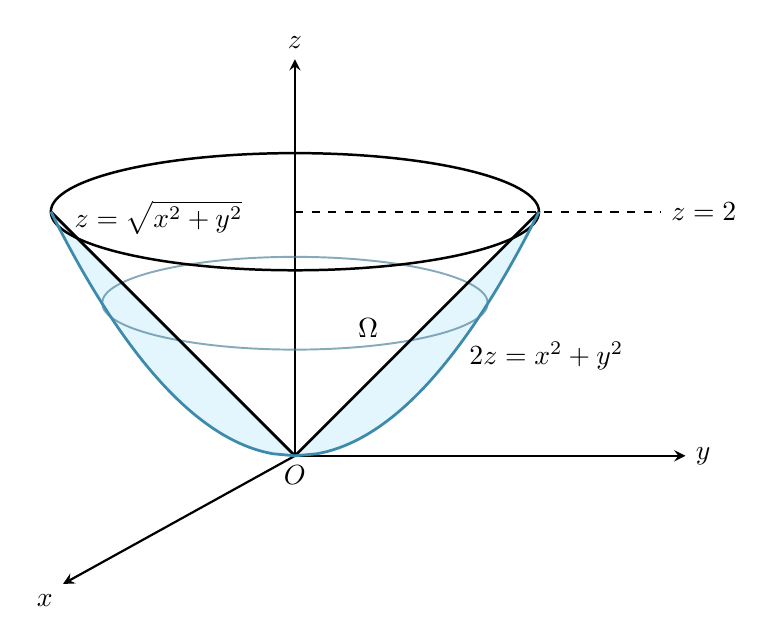
\begin{tikzpicture}[scale=1.55, >=stealth]
  % axes
  \draw[->, line width=0.8pt] (0,0) -- (3.2,0) node[right] {$y$};
  \draw[->, line width=0.8pt] (0,0) -- (0,3.25) node[above] {$z$};
  \draw[->, line width=0.8pt] (0,0) -- (-1.9,-1.05) node[below left] {$x$};

  % side shell region: only the two visible lateral sheets
  \fill[cyan!30, opacity=0.36]
    (0,0) -- (-2,2)
    -- plot[domain=2:0, samples=120] ({-sqrt(2*\x)}, \x)
    -- cycle;

  \fill[cyan!30, opacity=0.36]
    (0,0) -- (2,2)
    -- plot[domain=2:0, samples=120] ({sqrt(2*\x)}, \x)
    -- cycle;

  % interior reference ellipse
  \draw[cyan!55!black, line width=0.7pt, opacity=0.65] (0,1.25) ellipse (1.58 and 0.38);

  % intersection circle r = 2, z = 2
  \draw[line width=0.9pt] (0,2) ellipse (2 and 0.48);

  % cone outlines
  \draw[line width=1pt] (0,0) -- (2,2);
  \draw[line width=1pt] (0,0) -- (-2,2);

  % paraboloid outlines
  \draw[cyan!65!black, line width=1pt, domain=0:2, samples=120] plot ({sqrt(2*\x)}, \x);
  \draw[cyan!65!black, line width=1pt, domain=0:2, samples=120] plot ({-sqrt(2*\x)}, \x);

  % z=2 guide
  \draw[dashed, line width=0.8pt] (0,2) -- (3.0,2) node[right] {$z=2$};

  % labels
  \node[below] at (0,0) {$O$};
  \node at (0.6,1.05) {$\Omega$};

  \node[left] at (-0.35,1.95) {$z=\sqrt{x^2+y^2}$};

  \node[right] at (1.35,0.82) {$2z=x^2+y^2$};
\end{tikzpicture}
\end{document}
